%
% einleitung.tex -- Einführung
%
% (c) 2020 Prof Dr Andreas Müller, Hochschule Rapperswil
%
% !TEX root = ../../buch.tex
% !TEX encoding = UTF-8
%
\section{Einführung\label{geradlinig:section:einfuehrung}}
\kopfrechts{Einführung}
Mit Beginn der Industrialisierung zeigte sich, dass Rotationsbewegungen
mechanisch einfacher zu realisieren sind als geradlinige
Translationsbewegungen. Ein wesentlicher Grund dafür war, dass
geradlinige Bewegungen durch äussere Einflüsse wie Schwerkraft,
Reibung oder Fertigungsungenauigkeiten nur schwer präzise geführt
werden konnten. Aus diesem Grund etablierten sich Kreisbewegungen als
Grundlage zahlreicher Mechanismen und Antriebssysteme.
\index{Industrialisierung}%
\index{Rotation}%
\index{Translation}%
\index{Schwerkraft}%
\index{Reibung}%

Mit der fortschreitenden Industrialisierung stieg jedoch der Bedarf an
Mechanismen, die eine möglichst exakte geradlinige Bewegung erzeugen
konnten. Dies motivierte Ingenieure und Erfinder des 18. und
19.\,Jahrhunderts, sich intensiv mit der Entwicklung entsprechender
Mechanismen auseinanderzusetzen.

\subsection{Newcomens Dampfmaschine\label{geradlinig:subsection:newcomen}}
Eine der ersten Maschinen, welche mechanische Arbeit mithilfe einer
geradlinigen Kolbenbewegung verrichtete, war die von Thomas Newcomen im
\index{Newcomen, Thomas}%
Jahr 1712 entwickelte atmosphärische Dampfmaschine
\index{Dampfmaschine}%
\cite{wiki_newcomen}. Dabei wurde Wasserdampf in einen Zylinder
eingeleitet und anschliessend durch Einspritzen von kaltem Wasser
kondensiert. Dadurch entstand im Zylinder ein Unterdruck, sodass der
atmosphärische Druck den Kolben in den Zylinder drückte. Die dadurch
erzeugte lineare Bewegung wurde über 
einen Balancier\footnote{Als Balancier wird der zweiarmige Hebel an 
Dampfmaschinen bezeichnet.}
auf die gegenüberliegende Seite übertragen und zum Verrichten mechanischer
Arbeit genutzt.

Die Newcomen-Dampfmaschine gilt als die erste praktisch einsetzbare
Dampfmaschine und ist in Abbildung~\ref{fig:newcomen_engine}
dargestellt.
\begin{figure}
    \centering
    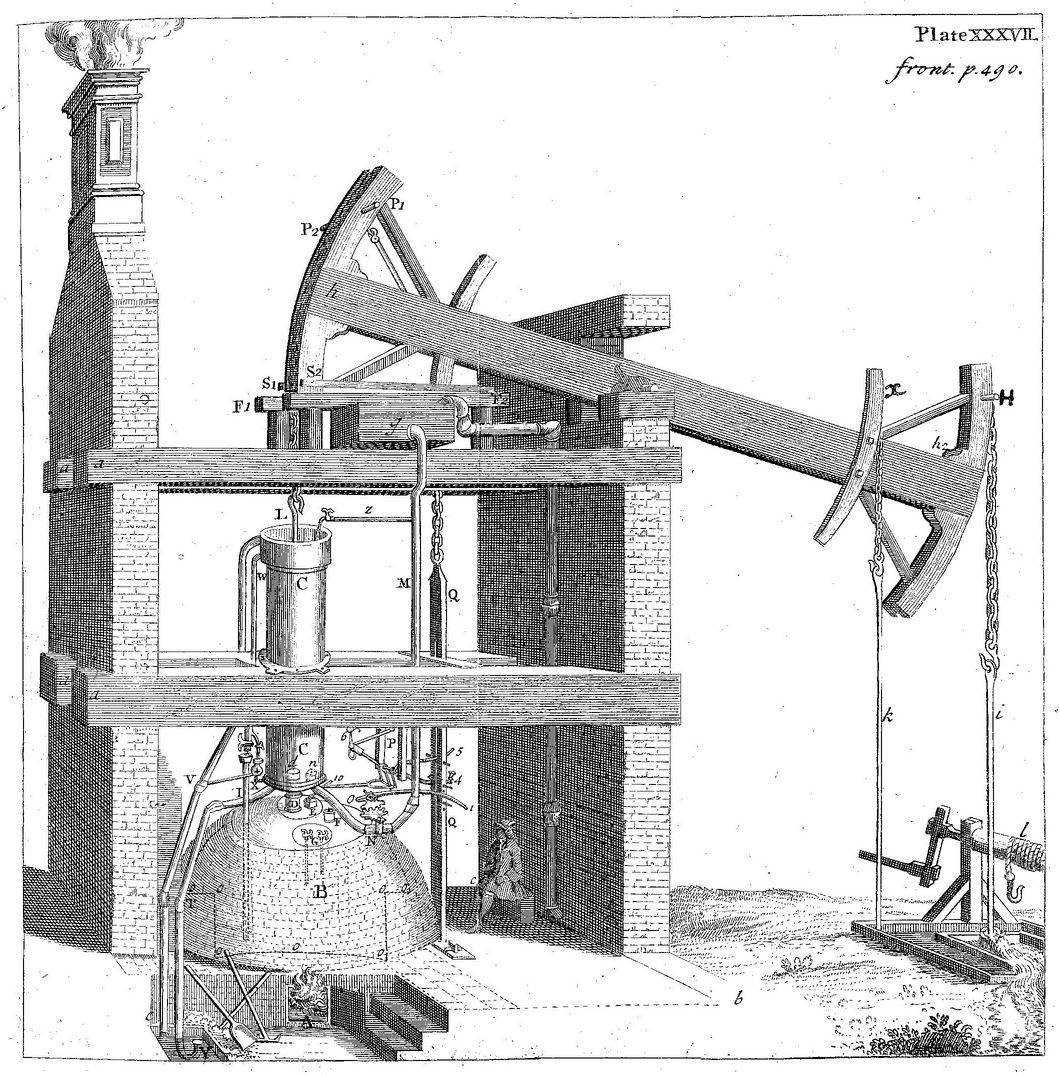
\includegraphics[width=\textwidth]{papers/geradlinig/figures/newcomen_engine.jpg}
    \caption{Illustration der Newcomen-Dampfmaschine~\cite{newcomen_pic}.}
    \label{fig:newcomen_engine}
\end{figure}


\subsection{Watts Dampfmaschine\label{geradlinig:subsection:watts_steam}}
James Watt erkannte das Potenzial, die Newcomen-Dampfmaschine zu verbessern.
\index{Watt, James}%
Insbesondere hielt er es für ineffizient, 
denselben Zylinder abwechselnd zu erhitzen 
und wieder abzukühlen~\cite{wiki_watt_steam}.
Deshalb ergänzte er die Maschine um einen separaten Kondensationszylinder.
Nachdem der Arbeitszylinder mit Dampf gefüllt war, 
wurde ein Ventil zum Kondensationszylinder geöffnet.
Der Dampf strömte in diesen und kondensierte dort.
Dadurch entstand derselbe Arbeitszyklus wie bei der 
Newcomen-Dampfmaschine, jedoch ohne den Arbeitszylinder nach jedem Hub abzukühlen.
Der Arbeitszylinder blieb dadurch heiss und war unmittelbar 
für den nächsten Arbeitshub bereit.
Später entwickelte Watt die Maschine zu einer doppeltwirkenden Dampfmaschine weiter.
Dabei wurde der Kolben abwechselnd von beiden Seiten mit Dampf angetrieben,
wodurch sowohl die Aufwärts- als auch die Abwärtsbewegung 
Arbeit verrichteten.
Die bisher verwendete Kette konnte hierfür nicht mehr 
eingesetzt werden und wurde durch eine starre Kolbenstange ersetzt.
Da sich die Kolbenstange geradlinig bewegte, der Balancier
jedoch um einen festen Drehpunkt schwenkte, 
war eine direkte Verbindung nicht möglich.
Aus diesem Grund entwickelte Watt den in 
Abbildung~\ref{fig:watts_engine} dargestellten Mechanismus.
Er kombinierte den Viergelenkmechanismus mit einem Pantographen, 
\index{Pantograph}%
um die Kolbenstange näherungsweise auf einer geraden Bahn zu führen.
\index{Kolbenstange}%
Diese Lösung war deutlich einfacher und kostengünstiger 
als eine präzise Linearführung.
Die verbesserte Kraftübertragung und die höhere Leistung machten 
die Maschine besonders geeignet zum Antrieb von Rädern.
\begin{figure}
    \centering
    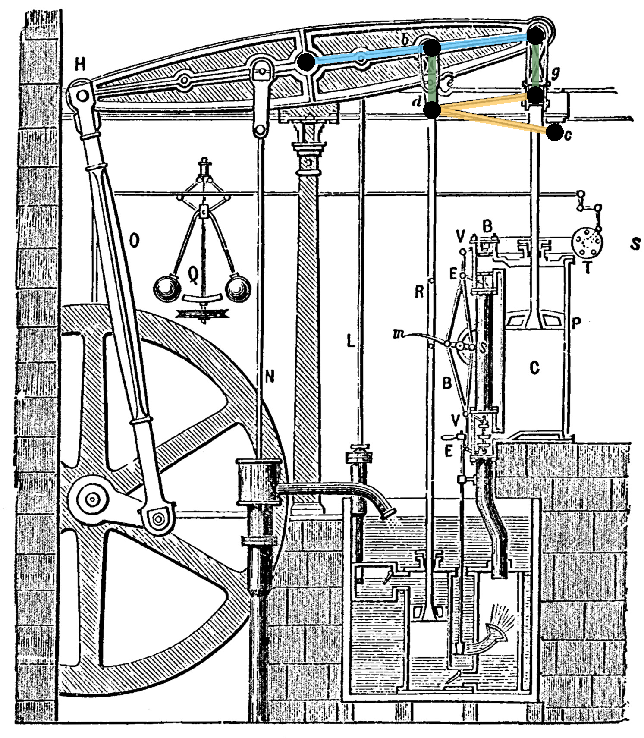
\includegraphics{papers/geradlinig/figures/watts-engine.pdf}
    \caption{Illustration der wattschen Dampfmaschine~\cite{wiki_watt_steam},
    welche den Mechanismus aus Abbildung~\ref{fig:watts_parallel_link} realisiert.}
    \label{fig:watts_engine}
\end{figure}


\subsection{Kinematische Synthese
\label{geradlinig:subsection:kinematische_synthese}}
\index{kinematische Synthese}%
Mit seiner Konstruktion legte James Watt den Grundstein 
für die \emph{kinematische Synthese}~\cite{kin_synth}.
Die kinematische Synthese beschreibt die systematische Entwicklung 
eines Mechanismus, der eine vorgegebene Bewegung erzeugt.
Dabei werden die Anordnung und die Abmessungen der 
einzelnen Glieder und Gelenke bestimmt.
Im Laufe der Zeit wurden zahlreiche Mechanismen entwickelt.
Einige dienten ausschliesslich der mathematischen Untersuchung, 
während andere in Maschinen und Fahrzeugen eingesetzt wurden.
Zu den einfachsten und wichtigsten Mechanismen 
gehört der Viergelenkmechanismus.
In diesem Paper werden ausschliesslich Mechanismen betrachtet, 
die durch Rotationsbewegungen eine approximative oder 
eine perfekte geradlinige Bewegung erzeugen.
